\ifdefined\included
\else
\setcounter{chapter}{0}
\dominitoc
\faketableofcontents
\fi

\chapter{Human Robot Collaboration Context}
\chaptermark{Human Robot Collaboration Context}
\label{chap:1}
\minitoc



%%%%%%%%%%%%%%%%%%%%%%%%%%%%%%%%%%%%%%%%%%%%%%%%%%%%%%%%%%%%%%%%%%%%%%%%%%%%%%%%%%%%%%
\section{Human-Robot Interaction}

This section is focused on general interaction between humans and robots and discuss related fields.

\subsection{Human-Human Interaction}

Many works dealing with interacting with humans take inspiration from human-human interaction. Human-Human interaction (HHI) refers to the communication and collaboration between two or more individuals, where humans engage in various forms of social, cognitive and emotional exchanges. Such interaction can occur through verbal and non-verbal communication, such as speech, gestures, facial expressions, and body language.

Hence, this field includes several studies such as communication theories, including non-verbal communication (Albert Meharbian's 7-38-55 rule, Shannon-Weaver model and Grice's maxims), social psychology (Stanley Milgram, Philip Zimbardo, and Solomon Asch), collaboration and teamwork (J.Richard Hackman, Amy C.Edmondson), conflict resolution and negotiation (Roger Fisher and William Ury), emotional intelligence (Daniel Goleman), cross-cultural communication.

HHI is a field that serves as an inspiration to design robots able to interact correctly with humans. Indeed, we must first understand how humans interact with each other, what is important to do and what should be avoided. Yet, mimicking humans perfectly is a questionable approach since robots and humans are fundamentally different. Robots should help and assist humans as tools. Such the way we interact with robot should be inspired by HHI but probably not similar.


\subsection{Human-Computer Interaction}

A first step of artificial interaction and collaboration is the field of Human-Computer Interaction. Human-Computer Interaction (HCI) is the field of study that focuses on optimizing how users and computers interact by designing interactive computer interfaces that satisfy users' needs. It is a multidisciplinary subject covering computer science, behavioral sciences, cognitive science, ergonomics, psychology, and design principles.
Today, HCI focuses on designing, implementing, and evaluating interactive interfaces that enhance user experience using computing devices. This includes user interface design, user-centered design, and user experience design. 

This field is made up of four key components. 
The User along with their needs, goals, interaction patterns, cognitive capabilities, emotions, and experiences.
The Goal-Oriented Task which is the objective or goal the user has in mind.
The Interface is about the overall user interaction experience through senses such as touch, click, gesture, voice, display size, colors.
The Context must be taken into account because it influences the interaction. 

To produce easy to interact with robots, the study of HCI is relevant and also serves as an inspiration to design intuitive, user-friendly interactive robots.

\subsection{Human-Robot Interaction}

Human-Robot Interaction (HRI) is a field of study that explores the design, development, and evaluation of robots that interact with humans in various settings. The goal of HRI is to create robots that can effectively and seamlessly collaborate with humans, whether in domestic environments, workplaces, or other contexts. It encompasses aspects of robotics, psychology, design, and engineering to understand and enhance the interactions between humans and robots.

Several subfields can be identified in HRI, here are some examples:
Social robotics focuses on social interactions with humans, and thus, explores how robots can understand and respond to human emotions, social cues, and communication styles.
Human-Centered Robotics emphasizes the importance of considering human needs and preferences. This subfield often involves user studies to ensure and identify if and how robots are user-friendly and can seamlessly integrate into human environments.
Robot ethics is another major subfield and is focused on considerations such as privacy, safety, responsibility/accountability and the impact of robots on society.
Explainable AI and transparency are a growing interest in making decision-making processes more understandable to humans, and thus, help robots be legible, predictable, and acceptable.
Collaborative robotics, or Cobots, focuses on developing robots that can work alongside humans in shared workspaces and usually as a team.
A significant amount of work is dedicated to HRI in Healthcare to assist patients, especially the elderly, and children with conditions. Those works are also usually linked to emotion-aware robotics which is focused on trying to recognize and respond to human emotions using affective computing techniques.   

As a subfield of HRI, Human-Robot Collaboration or Collaborative Robotics is still a vast subject which is worth to detail a bit more in the next section.

%%%%%%%%%%%%%%%%%%%%%%%%%%%%%%%%%%%%%%%%%%%%%%%%%%%%%%%%%%%%%%%%%%%%%%%%%%%%%%%%%%%%%%
\section{HRC Collaboration}

As mentioned above, Human-Robot Collaboration (HRC) refers to the synergy and cooperation between humans and robots in shared environments to achieve common goals. In HRC, humans and robots work together, often leveraging their complementary strengths to enhance overall performance and efficiency. This collaborative approach involves close interaction, communication, and coordination between human and robotic agents.

\subsection{Inspirations - Theories informing HRC}

This interdisciplinary field takes inspiration from various theories and field as introduced earlier. Yet, three main inspiration can be highlighted:

\subsubsection*{Belief Desire Intention Model:} The belief-desire-intention (BDI) model was originally developed by Michael Bratman [cite wikipedia]. This model is used in intelligent agents research to describe and model intelligent agents. Straightforwardly, the BDI model is characterized by the implementation of the three notions appearing in its name, i.e., an agent's beliefs (knowledge of the work in the perspective of the agent), desires (objective or goal to accomplish), and intentions (the planned course of actions to achieve the agent's desire). 

\subsubsection*{Shared Cooperative Activity:} Shared cooperative Activity defines prerequisites for an activity to be considered shared and cooperative. The main ones are mutual responsiveness, commitment to the joint activity and commitment to mutual support. A good example to clarify these prerequisites is a scenario where agents are moving a table together. Mutual responsiveness ensures that the agents' movements are synchronized. The commitment to the joint activity reassures each agent that the others will not drop their side and quit the joint activity. Finally, the commitment to mutual support deals with possible breakdowns due to one agent's inability to perform part of the plan.  

\subsubsection*{Joint Intention Theory:} Joint Intention Theory proposes that for joint action to emerge, team members must communicate to maintain a set of shared beliefs and to coordinate their actions towards the shared plan [cite]. In collaborative work, agents should be able to count on the commitment of other members, therefore each agent should inform the others when they conclude that a goal is achievable, impossible, or irrelevant [cite Hoffman].

\subsection{Key Aspects}

\textbf{Specialization of Roles:} There are several human-robot relationships including supervisor-subordinate, partner-partner, teacher-learner, and leader-follower. These roles can either be fixed and predefined, or there can be a flexible role distribution using weighting functions that allow a continuous change between the roles to adapt to every context and situation.

\textbf{Establishing shared goal(s):} Through direct discussion or inference, agents must determine the shared goals they are trying to achieve. However, a shared goal isn't always necessary and can be established in the middle of a task execution either by the human or the robot.

\textbf{Allocation of subtasks:} After deciding how to achieve their goals, agents must determine what actions and subtasks will be done by each agent and how to coordinate each other. This can either be done explicitly before starting the task or be reactively done on the fly.

\textbf{Progression tracking:} Agents must be able to track progress toward their goals. That is, they must be able to determine what has been achieved, by whom, and what remains to be done. 

\textbf{Communication:} Any collaboration requires communication, verbal or not. Most of the mentioned key aspects can or must involve communication.

\textbf{Adaption and learning:} On a short-term scale the agents must be able to adapt themselves to each other and the environment. On the longer term, agents must also learn from other partners and the acquired experience.

\textbf{Ergonomics:} Linked to HCI, it should be intuitive to collaborate and communicate with the robot. 

\subsection{Architecture - Complete system}

It is important to remember that since a collaborative robot is issued from an interdisciplinary field, the different functionalities and capabilities of the robot can usually be separated into several dedicated components. These components interact with each other in a complete architecture to exhibit the robot's behavior, from sensory perception to physical motions including reasoning processes. 
Hence, when working on a collaborative robot, it must be thought about as a whole and each aspect cannot be studied completely indecently from all other aspects of the complete system. 

Some works are dedicated to designing robotic architectures, especially cognitive architectures which are the closer/best have found to design collaboration robots. 

Example of cognitive architecture
[cite SOAR Laird et al, CORTEX Bustos et al, ORO/SHARY/SPARK.. Lemaignan, perspective-aware Lemaignan]

%%%%%%%%%%%%%%%%%%%%%%%%%%%%%%%%%%%%%%%%%%%%%%%%%%%%%%%%%%%%%%%%%%%%%%%%%%%%%%%%%%%%%%
\section{Navigation}

Human-aware navigation is the intersection between research on human-robot interaction (HRI) and robot motion planning.

As stated in \cite{thesisBuisan21}, robot navigation aims to make the robot base (the whole robot) move from one place to another while avoiding static and moving obstacles. However, when the robot has to move in an environment where humans are evolving, other constraints must be added. 
Humans shouldn't just be avoided as other moving obstacles and their psychological and mental state must be taken into account. Hence, the robot neither should move threateningly, block the humans, nor induce drastic changes in their motion. Taking all these aspects into account is what is called human-aware robot navigation.

One of my contributions is to propose a simulated human agent endowed with decision-making processes dedicated to navigation in order to challenge human-aware robot navigation systems. To do so, the simulated avatar also uses some human-aware navigation techniques. Hence, I briefly describe in this section the current robot navigation techniques and some existing benchmarking tools used in robot navigation to show the lack of such intelligent simulated agents.

\subsection{Robot Navigation techniques}

State-of-the-art techniques for robot navigation involve two kinds of motion planners: a global and a local planner. The global planner is in charge of finding the best overall trajectory leading the robot to its goal, producing a global plan. This planner usually only takes into account static obstacles described by a given map of the environment. Then, the local planner is in charge of producing velocity commands sent to the motor controllers to follow the produced global plan. To produce the velocity commands the local planner may produce a local plan with only a few seconds of time horizon that follows the global plan while taking into account obstacles detected in real-time by the robot sensors, including moving obstacles. This way the robot should reach its goal while being reactive to moving obstacles. 

Recent techniques also involve learning methods.

However, how explained above, such approaches are not sufficient in human-populated environments. Humans must be detected and treated differently during the motion planning process. Human-aware approaches detect and track nearby humans and try to estimate their trajectory to plan the robot one accordingly. This is achieved in works like [cite CoHAN] where the human trajectory is estimated using goal recognition processes and elastic bands methods. Then, the robot's motion is planned using also elastic band methods that are tuned to take into account the robot's goal, the estimated human trajectory and other social norms.   

\subsection{Benchmarking tools and metrics}

Where it is easy to benchmark robot navigation on objective metrics like the time to reach a goal, the distance traveled and the number of collisions [cite BARN Perille], it is more challenging to benchmark their human-aware properties.
First, there is no consensus on the metrics to use to evaluate the human-aware properties of a navigation system. State-of-the-art metrics involve proxemics [cite]. Yet, other metrics can be relevant such as the deviation imposed to the human motion, and the feeling of threat produced.
Also, it is challenging to find a usable system that will effectively challenge a HAN system. 
Common approaches involve reactive-only techniques such as social force models. Such reactive models are easy to use and efficient for crowd simulations, but in intricate scenarios involving some decision-making they can perform very poorly. Thus, there was a lack of intelligent simulated agents to challenge effectively HAN system.
I started to work on this aspect in 2020. Now, a few recent work also propose to simulate human agent endowed with some reasoning processes but I didn't find the time to properly compare my contribution with them. Yet, this shows that this is a subject of interest and a few a such work can be mentioned here. Some related works will be discussed in Chapter~\ref{chap:6}.


%%%%%%%%%%%%%%%%%%%%%%%%%%%%%%%%%%%%%%%%%%%%%%%%%%%%%%%%%%%%%%%%%%%%%%%%%%%%%%%%%%%%%%
\section{Models for interaction}

\textbf{For now, mostly from Buisan thesis}

% In this section are introduced some notations and task modeling approaches relevant for the human-robot interaction. The purpose of this section is to clarify both the different models used, especially from which perspective, and the basics task modeling that will be used throughout all this thesis.


It has been shown previously that a robotic agent interacting with a human needs to coordinate its actions with them [cite?]. Moreover, joint action theory exhibits that humans interacting together represent the task as a whole, and plan not only for their actions but also for the actions of other agents. Thus, we think that for a human to perform the most efficient and satisfactory joint task with a robot, this robot must explicitly model human actions and plan not only for its actions but also for the human ones. This is why we present in this section some notations to clarify the different models used in this thesis, and then we present in more details how to model tasks.

\subsection{Human and Robot agents}

\begin{figure}
    \centering
    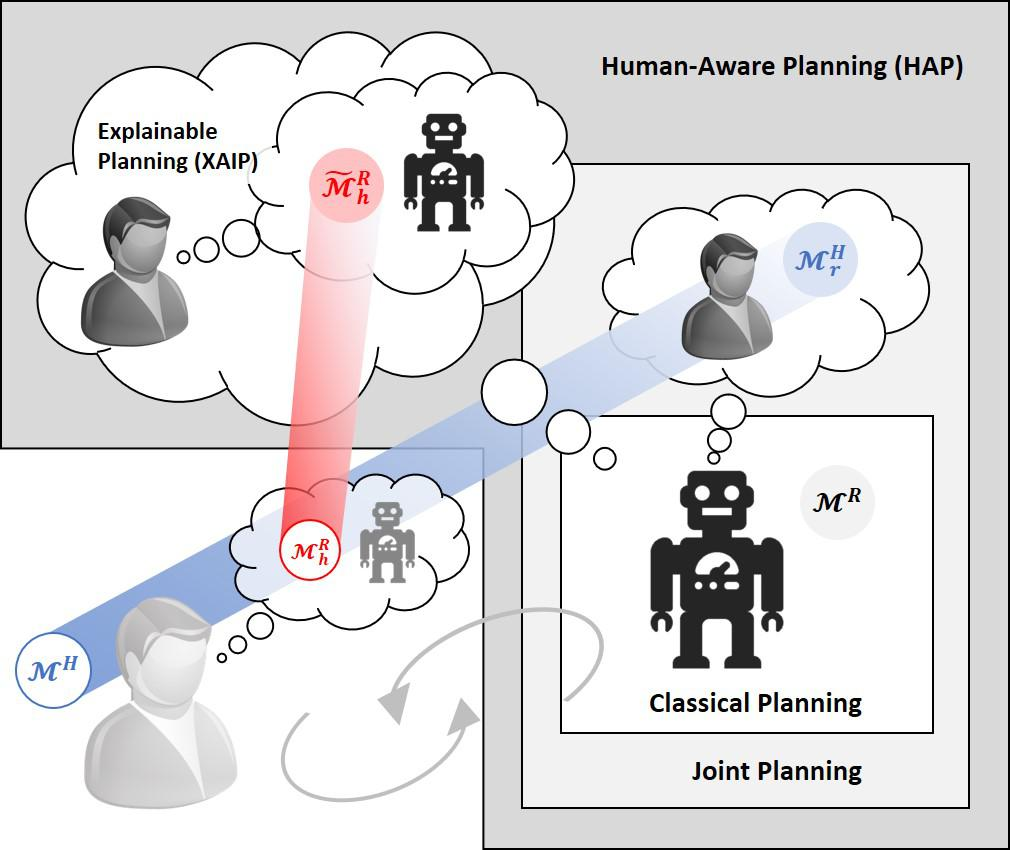
\includegraphics[width=0.8\linewidth]{images/Chapter1/chakraborti_notations.jpg}
    \caption{Agent models from Chakraborti \textit{et al.} notations.}
    \label{fig:chakraborti_notations}
\end{figure}

Chakraborti \textit{et al.} introduced notations to differentiate between the models used in this thesis in their work~\cite{ChakrabortiBTZS15}, also used in Buisan's thesis~\cite{thesisBuisan21}. These notations summarize and differentiate elegantly the different models manipulated in the HRI/HRC field. These notations are depicted in figure~\ref{fig:chakraborti_notations}. At the bottom are depicted the human agent (on the left) and the robot agent (on the right). When solving a task alone, the robot uses its own model referred to as $\mathcal{M}^R$ and this is considered as Classical Planning. 
Then, $\mathcal{M}^H_r$ is an estimation by the robot of the model of the human. Finally, $\tilde{\mathcal{M}}^R_h$ is an estimation of the robot model the human has. 

It is important to keep in mind that when discussing a task planner it is considered as part of the robot. Thus, $\mathcal{M}^R$ is considered as the ground truth for the robot. As a consequence, if there is a belief divergence between $\mathcal{M}^H_r$ and $\mathcal{M}^R$, we always consider that $\mathcal{M}^R$ is the truth, otherwise, it would make no sense to keep this information in $\mathcal{M}^R$ while having access to the one in $\mathcal{M}^H_r$.

\subsection{Task modeling}

A common way of representing human activity (MrH ) and interaction with computers at a high abstraction level is by using task models. The hierarchical structure of human activity was first exploited by Annett and Duncan [Annett 1967]. They state that tasks can be described at several levels of abstraction until a certain criterion is met. Each task can thus be refined into subtasks detailing the procedure followed by the human to achieve the higher level task. Task modeling has then evolved to introduce interaction with systems, produced and needed information, potential errors and a wide variety of operator specifying how tasks interact with each other during their execution. Task models are now commonly used in user-centered and user-interface design processes. Most advanced notations include ConcurTaskTrees [Paternò 2004] and HAMSTERS [Martinie 2019]. These models are used to design or evaluate interactive systems. They allow the designer to better understand the user task or to study the user workflow using their system. However, these models contain too little information for a system to be able to reason and make decisions on them (either in planning or acting).


\subsection{Hierarchical models}

In classical planning, each action of an agent is atomic and needs some conditions to hold in the environment to be executed, then it changes the environment when applied. The planning process has then to find the right sequence of actions, being applicable one after the other to change the environment to reach a certain goal state. 
However, it has been shown (cite?) that humans tend to plan their actions differently. Indeed, we usually work on a more abstract level and tend to decompose tasks hierarchically into small tasks until reaching the action level. In practice, using Hierarchical Task Networks (HTNs) allow the domin designer to help the plan search by inserting expert knowledge via a hierarchy linking the actions [erol 1996]. A task network consists in tasks organized in a fully or partially ordered manner, and each task can be either abstract or primitive. Primitive tasks are elementary tasks that can be achieved by performing one associated action. On the other hand, abstract tasks are tasks that first need to be decomposed into other subtasks, ``more primitive". The goal of the planner is not to find the sequence of actions to reach a goal, but rather to select recursively for each task the right decomposition ending (if possible) with a network of actions applicable from the initial state. Such a process is named by Ghallab, Nau and Traverso as planning with refinement methods [Ghallab 2016]. This planning hierarchy not only allows the domain designer to guide the search by inserting some expertise into the model, but also to enhance explainability as the decompositions often offer a semantic to their subtasks (the why can usually be answered by going up in the hierarchy, while the how is answered by going down. 

%%%%%%%%%%%%%%%%%%%%%%%%%%%%%%%%%%%%%%%%%%%%%%%%%%%%%%%%%%%%%%%%%%%%%%%%%%%%%%%%%%%%%%
\section{Task Planning}

\subsection{Classical Planning}

As put by Ghallab, Nau and Traverso, “the purpose of planning is to synthesize an organized set of actions to carry out some activity” [Ghallab 2016]. 
Classical planning is a type of planning that assume deterministic and fully observable environments. It involves representing the world as a set of states and actions, with plans derived through state space search algorithms. Actions have preconditions and effects, and planning problems entail finding a sequence of actions transforming an initial state into a goal state. Classical planning algorithms, including STRIPS, Graphplan, and Fast Downward, utilize heuristics to guide the search efficiently. While well-suited for domains with clear and deterministic dynamics, classical planning may face challenges in handling uncertainty or partial observability, leading to the development of alternative planning approaches for such scenarios.

\subsection{Planning for HRC}

Classical planning has been vastly studied and can now solve efficiently various problems. Yet, the intricate nature of HRC scenarios demands sophisticated task-planning methodologies capable of adapting to dynamic environments, understanding human intent, and promoting a fluent exchange of information. Hence, several subfields of task-planning have emerged and are used in HRC. Here are a few examples:

\begin{itemize}
    \item \textbf{Hierarchical Task Planning} is a technique that organizes tasks in a hierarchical structure like presented in the previous section, allowing for the representation of complex tasks at various abstraction levels. This approach enhances modularity, flexibility and explainability in task planning, accommodating intricate collaborative scenarios.
    
    \item \textbf{Mixed-Initiative Planning} leverages the strengths of both humans and robots by allowing for a dynamic allocation of decision-making authority. This technique promotes collaborative decision-making, enabling the system to adapt to the expertise and preferences of each agent involved in the collaborative task.
    
    \item \textbf{Human-Centric Task Planning} focuses on incorporating human factors into the planning process. This involves understanding human capabilities, preferences, and cognitive load to optimize task plans that align with the natural workflows and expectations of human collaborators.
    
    \item \textbf{Learning-Based Task Planning} has emerged thanks to advancements in machine learning as a frontier in adapting to evolving environments. This technique involves training models to understand patterns in human behavior, enabling the robot to learn and adapt its task planning strategies over time. Such techniques can also be used to predict human behavior and adapt the robot's actions consequently.
    
    \item \textbf{Probabilistic Task Planning} integrates uncertainty into the planning process, acknowledging the inherent unpredictability of human behavior and environmental factors. By incorporating probabilistic models, this technique enhances the robustness of task plans in dynamic and uncertain collaborative settings.
\end{itemize}

Overall, \textbf{Human-Aware Task Planning} is the process of considering the presence and behavior of humans in the planning and execution of robot tasks. It involves taking into account cues from the shared environment and the dynamics of human-robot interaction. The goal is to generate robot policies that are adaptable, robust, and efficient in crowded and dynamic environments. This field includes having an explicit shared task or common goal between the human and the robot, implying that the two agents will collaborate to reach the goal. It also includes not having an established shared goal, and thus, is closer to what I would call an interaction instead of a collaboration. Yet, both problems are interesting and must be addressed, with a unified approach or not. 
The approaches presented in this thesis are in between the first three subfields listed above. 


